\section{Рабочий проект}
\subsection{Классы, используемые при разработке сайта}

Можно выделить следующий список классов и их методов, использованных при разработке интеллектуальной системы (таблица \ref{class:table}).

\renewcommand{\arraystretch}{0.8} % уменьшение расстояний до сетки таблицы
\begin{xltabular}{\textwidth}{|X|p{2.5cm}|>{\setlength{\baselineskip}{0.7\baselineskip}}p{4.85cm}|>{\setlength{\baselineskip}{0.7\baselineskip}}p{4.85cm}|}
\caption{Описание классов и методов системы\label{class:table}}\\
\hline \centrow \setlength{\baselineskip}{0.7\baselineskip} Название класса & \centrow \setlength{\baselineskip}{0.7\baselineskip} Модуль, к которому относится класс & \centrow Описание класса & \centrow Методы \\
\hline \centrow 1 & \centrow 2 & \centrow 3 & \centrow 4\\ \hline
\endfirsthead
\caption*{Продолжение таблицы \ref{class:table}}\\
\hline \centrow 1 & \centrow 2 & \centrow 3 & \centrow 4\\ \hline
\finishhead
Database\-Manager & database\-Manager & DatabaseManager -- класс для управления подключением к базе данных PostgreSQL и выполнения запросов для получения данных о болезнях томатов & get\_connection() создает и возвращает соединение с базой данных, используя параметры конфигурации из Config;

get\_disease(string disease\_name) извлекает из базы данных описание болезни, методы её лечения и меры профилактики по её названию, возвращает словарь с данными, если болезнь найдена. \\

\hline
ImagePro\-cessor & imagePro\-cessor & ImageProcessor -- класс для подготовки изображений к анализу моделью. & preprocess\_image(ima\-ge) изменяет размер изображения, улучшает контрастность, резкость и яркость, чтобы подготовить его к анализу моделью, возвращает обработанное изображение.

resize\_for\_display(ima\-ge) изменяет размер изображения до фиксированного для отображения на веб-странице, возвращает изменённое изображение;

convert\_to\_base64(ima\-ge) преобразует изображение в строку base64 для передачи и отображения в веб-приложении, возвращает закодированную строку. \\

\hline
TomatoDi\-seaseModel & model & TomatoDiseaseModel – класс для загрузки модели YOLO и выполнения предсказаний болезней томатов на основе изображений; & predict(img\_input) анализирует входное изображение с помощью модели YOLO и возвращает название обнаруженной болезни и уверенность в предсказании, или сообщение о проблеме. \\

\hline
YOLOTrai\-ner & trainModel & YOLOTrainer – класс для обучения и оценки модели YOLO для обнаружения болезней томатов. & train() выполняет обучение модели YOLO на заданном наборе данных с указанными параметрами, возвращает результаты обучения; 
test() Проводит оценку модели на тестовом наборе данных, возвращает результаты оценки;
predict(source) выполняет предсказание по изображению, возвращает результаты предсказания. \\

\hline
YOLOv11In\-ference & trainModel & YOLOv11Inference – класс для выполнения инференса модели YOLOv11 на изображениях и визуализации результатов & run(image\_dir) выполняет инференс на случайных изображениях из указанной директории, отображает результаты с рамками и метками, возвращает список словарей с данными предсказаний; predict\_single(ima\-ge\_path) выполняет инференс на одном изображении, возвращает словарь с данными предсказания, включая рамки, метки и уверенности.\\

\end{xltabular}
\renewcommand{\arraystretch}{1.0} % восстановление сетки

\subsection{Обучения модели}

\subsubsection{Описание датасета}

Обучение и тестирование модели проводились на специально подготовленном датасете, содержащем изображения здоровых растений и листьев томатов с признаками различных заболеваний. Общее количество изображений равно 18612. В датасете 70\% используется для обучения, 20\% для валидации и 10\% для тестирования. Изображения приводятся к размеру 640x640 пикселей. Большая часть данных была взята из открытого датасета plantvillage, остальные фото были найдены в сети интернет.

Датасет был подготовлен с использованием разметки в формате YOLO, где каждое изображение сопровождается аннотацией с координатами ограничивающих рамок и метками классов. 

Для улучшения качества модели применялись методы аугментации данных, такие как повороты и изменения яркости, что позволило увеличить разнообразие обучающей выборки.

\subsection{Результаты обучения}

Обучение модели проводилось на платформе Google Colab с использованием графического процессора. Обучение проводилось на протяжении 100 эпох с размером пакета равным 16. Начальная скорость обучения равна 0.001. Для оптимизации использовался оптимизатор AdamW. Коэффициент импульса равен 0.937. Снижение веса установлено в 0.0005.

Графики на рисунке~\ref{fig:results} отражают динамику метрик в процессе обучения. На оси $x$ отложены эпохи (от 1 до 100), а на оси $y$ -- значения метрик.

\begin{figure}[H]
	\centering
	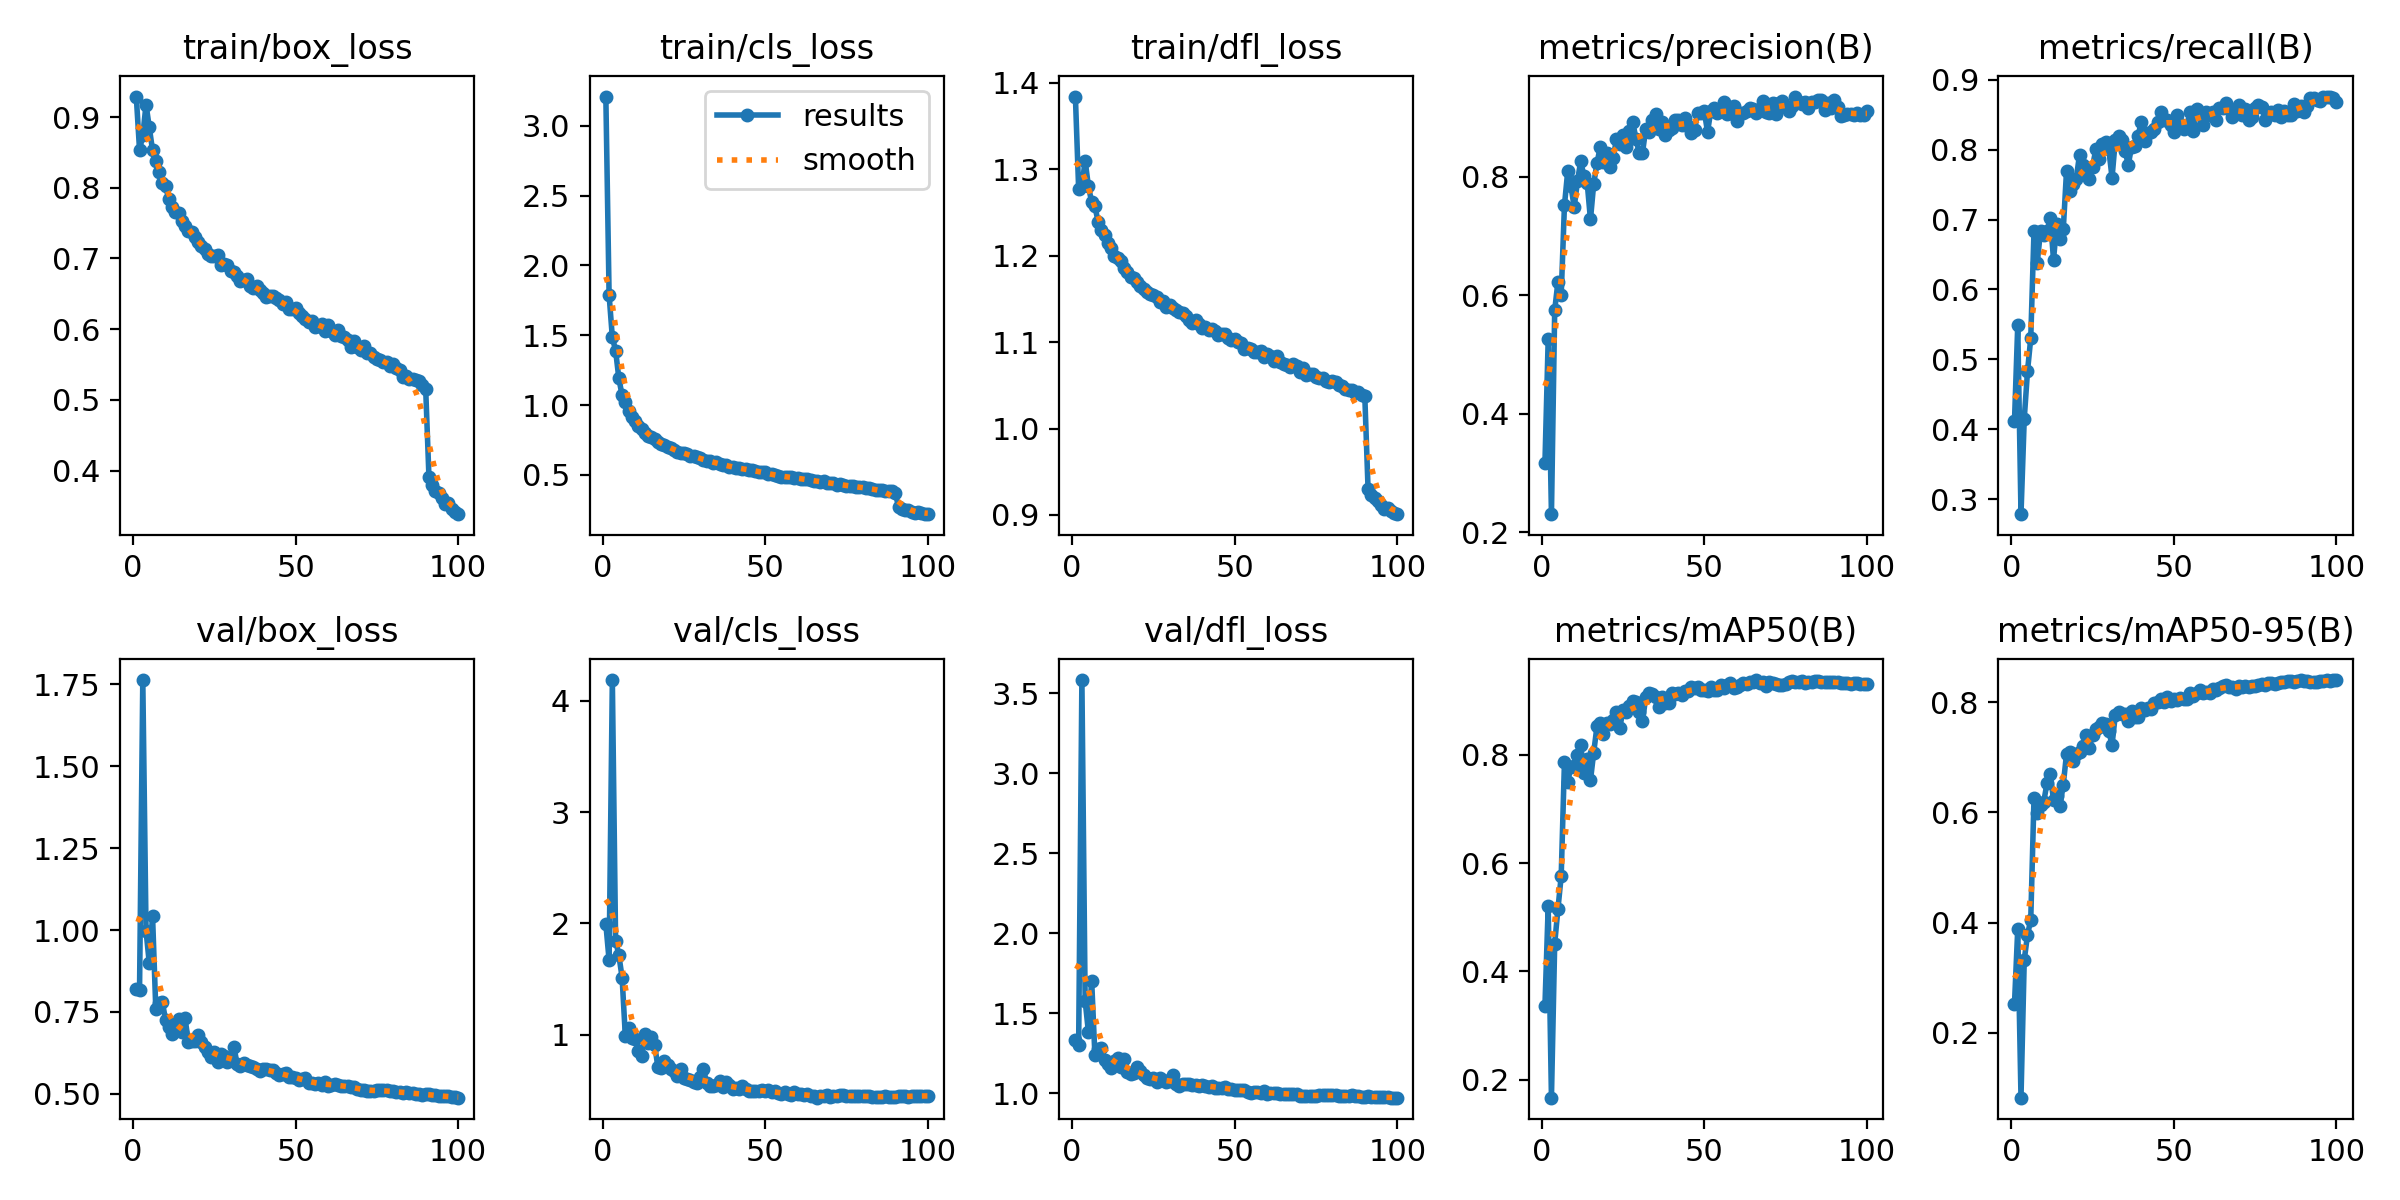
\includegraphics[width=1\textwidth, height=0.65\linewidth]{results.png}
	\caption{Динамика метрик обучения.}
	\label{fig:results}
\end{figure}

Box Loss (train/val) показывает потери на ограничивающие рамки, то есть насколько точно модель обводит больные участки листьев. На старте потери были высокими: больше 0.9 для обучающего набора и 1.75 для валидационного. Но к 50-й эпохе они снизились до 0.6 (train) и 0.6 (val), а к концу обучения, на 100-й эпохе, достигли 0.3 и 0.5 соответственно. Это говорит о том, что модель стала гораздо точнее определять местоположение поражённых зон.

Class Loss (train/val) отражает потери классификации. В начале они превышали 3 при обучении и 4 при валидации, но уже к 30-й эпохе упали до 0.7 и 0.6 соответственно. К 100-й эпохе значения снизились, примерно, до 0.2 при обучении и 0.3 при валидации. Можно сделать вывод, что модель научилась уверенно определять болезни на фото.
 
Dfl Loss (train/val) показывают, как изменялись потери, связанные с распределённой фокальной функцией потерь (dfl Loss), которая отвечает за точное определение формы и размеров ограничивающих рамок вокруг больных участков листьев. В начале они составляли 1.4 при обучении и 3.5 при валидации. К 30-й эпохе значение снизилось до 1.1 и 1.2. К концу обучения значения снизились до, примерно, 0.9 при обучении и 1 при валидации. Это говорит о том, что модель научилась более точно подгонять рамки под форму и размеры больных участков.

Precision(точность) иллюстрирует, насколько часто модель правильно классифицирует больные участки листьев, избегая ложных срабатываний. На старте точность была низкой -- около 0.2, что говорит о значительном количестве ошибок. Однако уже к 20-й эпохе значение выросло до 0.6, а к 50-й -- до 0.8. К 80-й эпохе точность стабилизировалась на уровне 0.85, оставаясь на этом уровне до конца обучения. Это указывает на то, что модель научилась с высокой уверенностью определять болезни.

Recall(полнота) показывает, насколько успешно модель обнаруживает все случаи заболеваний. Начальное значение было около 0.3. К 50-й эпохе полнота поднялась до 0.8. К концу обучения она достигла 0.88. Это говорит о том, что модель стала эффективно находить почти 88\% всех больных участков.

mAP50 отражает среднюю точность классификации при пороге пересечения IoU равного 0.5. На первой эпохе mAP50 был меньше 0.2. К 20-й эпохе значение выросло до 0.6, а к 50-й — до 0.83. К 80-й эпохе mAP50 стабилизировался на уровне 0.88. Данный результат подтверждает высокую способность модели правильно классифицировать заболевания.

mAP50-95 учитывает среднюю точность при порогах IoU от 0.5 до 0.95, оценивая как классификацию, так и точность локализации. Начальное значение было около 0.15, но к 20-й эпохе оно стало больше 0.6, а к 50-й -- превысило 0.7. К 100-й эпохе mAP50-95 поднялся до 0.8. Это показывает, что модель не только верно определяет болезни, но и достаточно точно обводит поражённые области, даже при высоких требованиях к точности.

В целом, данные результаты свидетельствуют об успешном процессе обучения модели, демонстрируя постепенное повышение ключевых показателей эффективности на протяжении всех итераций.



\subsection{Системное тестирование}

